\chapter{Further Properties of the Correspondence}
\label{chap:further_properties}

\chapterquote{Everything is  funny,  if you can laugh at it.}{Lewis Carroll}

The previous chapter introduced the graph-simplex correspondence and devoted several sections to the basic properties of the simplices associated to a given graph. In this chapter we  continue the study of the correspondence and present several of its more significant (but perhaps more complicated) properties.  We begin,  however, by demonstrating that  some of the interplay between $\splx_G$ and $\splx_G^+$ generalizes to an arbitrary simplex and its dual. 

\section{A General Property of the Dual Simplex }
Given that $\splx_G^+$  is the dual of $\splx_G$, it is natural to wonder whether some aspects of  their relationship are common to that between any simplex and its dual.  
Here we demonstrate that this is indeed the case; in particular, the Gram matrix of any (centred) simplex and its dual enjoy  the same pseudoinverse relationship. 
As we explained in Section~\ref{sec:Sn_G}, this relationship  is crucial to many of the proofs pertaining to  the combinatorial  simplices.
That  an equivalent property  holds for arbitrary simplices is therefore highly beneficial for their  study. 

\begin{lemma}
	\label{lem:dual_pseudoinverse}
	Let $\ssplx\subset\R^{n-1}$ be an arbitrary centred  simplex, and $\ssplx^\du$ its dual. Put $\Sv=\Sv(\ssplx)=(\bgamma_i)$ and $\Sv^\du=\Sv(\ssplx)=(\bgamma_i^\du)$ as usual. Then $\Sv^\du\Sv^\tp = \Sv(\Sv^\du)^\tp=\I$ and $(\Sv^\du)^\tp\Sv^\du$ is the Moore-Penrose pseudoinverse of $\Sv^\tp\Sv$. 
\end{lemma}
\begin{proof}
	First we inquire into the relationship between $\Sv$ and $\Sv^\du$. Put $\M=(\bgamma_1-\bgamma_n,\dots,\bgamma_{n-1}-\bgamma_n)$ and $\Q = (\bgamma^\du_1,\dots,\bgamma_{n-1}^\du)$. By definition, $\{\bgamma_i^\du\}$ is the dual  basis to $\{\bgamma_i-\bgamma_n\}$. Thus, by Observation~\ref{obs:bi-orthogonal_unique}, $\Q^\tp=\M^{-1}$ (we are working in $\R^{n-1}$), so  $\M\Q^\tp=\I$. The $(i,j)$-th component of this matrix product can therefore be expressed as 
	\begin{align}
	\delta_{ij} = \M\Q^\tp(i,j) &= \sum_{\ell=1}^{n-1} (\bgamma_\ell(i) - \bgamma_n(i))\bgamma_\ell^\du(j) = \sum_{\ell=1}^{n-1} \bgamma_\ell(i)\bgamma^\du_\ell(j) - \bgamma_n(i)\sum_{\ell=1}^{n-1}\bgamma^\du_\ell(j).\label{eq:lem_dual_pseudoinverse1}
	\end{align}
	Now,  since $\ssplx^\du$ is centred, 
	\begin{equation*}
	0=	(\Sv^\du\one)(j) = \sum_{\ell\in[n]} \bgamma_\ell^\du(j),
	\end{equation*}
	implying that $\sum_{\ell=1}^{n-1}\bgamma_\ell^\du(j) = - \bgamma_n^\du(j)$. Equation~\eqref{eq:lem_dual_pseudoinverse1} can then be written as 
	$
	\sum_{\ell=1}^{n} \bgamma_\ell(i)\bgamma_\ell^\du(j)=\delta_{ij},
	$
	implying that the components of $\Sv^\du\Sv^\tp$ are
	\begin{align*}
	(\Sv^\du\Sv^\tp)(i,j) &= \sum_{\ell=1}^n \bgamma_\ell^\du(i)\bgamma_\ell(j)=\delta_{ij},
	\end{align*}
	so that $\Sv^\du\Sv^\tp=\I$. A similar argument  holds for $\Sv(\Sv^\du)^\tp$, \emph{mutatis mutandis}.  
	
	We now proceed to demonstrating the pseudoinverse relation between $\Sv^\tp\Sv$ and $(\Sv^\du)^\tp\Sv^\du$. Recall that to demonstrate that  a matrix $\B_1$ is the pseudoinverse of $\B_2$, we need  to show that (i) $\B_1\B_2\B_1=\B_1$, (ii) $\B_2\B_1\B_2=\B_2$, (iii) $(\B_1\B_2)^\tp = \B_1\B_2$ and  (iv)  $(\B_2\B_1)^\tp = \B_2\B_1$ (Definition~\ref{def:simplex}). Using the relationship between  $\Sv^\du$ and  $\Sv$ given above, these become simple computations. For instance, 
	\begin{equation*}
	\Sv^\tp\Sv(\Sv^\du)^\tp\Sv^\du\Sv^\tp\Sv = \Sv^\tp \I^2 \Sv=\Sv^\tp\Sv,
	\end{equation*}
	and, 
	\begin{align*}
	((\Sv^\du)^\tp\Sv^\du \Sv^\tp\Sv)^\tp = ((\Sv^\du)^\tp\I\Sv)^\tp = \Sv^\tp\Sv^\du = \I-\frac{\J}{n} = (\Sv^\du)^\tp\Sv = (\Sv^\du)^\tp\I\Sv = (\Sv^\du)^\tp\Sv^\du\Sv^\tp\Sv.
	\end{align*} 
	Conditions (i) and (iii) therefore  hold between $\Sv^\tp\Sv$ and  $(\Sv^\du)^\tp\Sv^\du$; conditions (ii) and (iv) follow similarly. 
\end{proof}


In the next  section, we  will demonstrate  that this insight allows us to  generalize results pertaining to hyperacute simplices to all simplices. 
We thus witness another benefit of the correspondence: By leveraging knowledge  of $\splx_G$ and $\splx_G^+$ we  can  gain insights into the behaviour of general simplices. 



\section{Block Matrix Equations}
\label{sec:block_matrix}
In this section we are finally able  to satisfy those readers who have  wondered about the applicability of electrical  networks to the graph-simplex correspondence. Applying Lemma~\ref{lem:block_equation_graph}, we are able to  develop block matrix equations which relate the structure of $\splx_G$ and $\splx_G^+$. Then,  using the results of the previous section we generalize  these equations to arbitrary simplices.  

Before we  begin, a brief remark on the relationship of the following results  and Fiedler's work. Fiedler's derivation of the graph-simplex correspondence relied on a matrix equation---an equation equivalent to~\eqref{eq:simplex_block_matrix}, in fact~\cite[Theorem 3.1]{fiedler1993geometric}. Conversely, we are obtaining such equations as a \emph{consequence} of the correspondence. It is our hope that different treatments of the material shed light on its different---and hopefully complementary---implications.  

Let a centred, hyperacute simplex $\ssplx$ be given, with $\Sv(\ssplx)=\{\bgamma_i\}$.  Let $\bar{d}$ be the average squared distance between all the vertices of $\ssplx$, that is
\begin{equation}
\label{eq:avg_squared_distance}
\bar{d} \equiv  \frac{1}{n^2}\sum_{i\leq j} \norm{\bgamma_i-\bgamma_j}_2^2.
\end{equation}
Let $\xi(i)$ give the average squared distance of vertex $i$ from other vertices minus the total average distance, 
\begin{equation}
\label{eq:avg_sqd_distance_i}
\xi(i) \equiv \frac{1}{n}\sum_{j} \norm{\bgamma_i-\bgamma_j}_2^2 - \bar{d},
\end{equation}
and put $\bxi=(\xi(1),\dots,\xi(n))$. 
The following  results relate  the distance matrix of $\ssplx$ to the vertex  matrix of its dual. 

\begin{lemma}
	\label{lem:block_inverse_simplex}
	Let $\ssplx\subset\R^{n-1}$ be a hyperacute simplex with  squared distance matrix $\D_\ssplx$, and average squared distance vector $\bxi$.
	Let $\Q=(\Sv^\du)^\tp\Sv^\du$  where $\Sv^\du$ is the vertex matrix of $\ssplx^\du$.  Then, 
	\begin{equation}
	\label{eq:simplex_block_matrix}
	-\frac{1}{2} \begin{pmatrix}
	0 & \one_n^\tp \\ 
	\one_n &  \D_\ssplx
	\end{pmatrix} = \begin{pmatrix}
	\bxi^\tp \Q\bxi + 4\overline{d} & -(\Q\bxi + 2\one/n)^\tp \\
	-(\Q\bxi + 2\one/n) & \Q
	\end{pmatrix}^{-1}.
	\end{equation}
	Moreover, the vertices of $\ssplx^\du$ and the distance matrix of $\ssplx$ are related by the equation
	\begin{equation}
	\label{eq:lem_inverse_relation}
	\Q \D_\ssplx \Q = -2\Q,
	\end{equation}
	and in the space $\spn(\one)^\perp$ it holds that 
	\begin{equation*}
	\label{eq:lem_inverse_relation2}
	\D_\ssplx\Q \D_\ssplx= -2\D_\ssplx.	
	\end{equation*}
\end{lemma}

\begin{proof}
By Theorem~\ref{thm:graph-simplex}, $\ssplx$ is the inverse simplex of some graph $G$ and therefore $\D=\D_\ssplx=\Reff$, where $\Reff$ is the effective resistance matrix (Lemma~\ref{lem:S_G_basic_properties}). Therefore, we can rewrite $\xi(i)$ as 
 \begin{align*}
\frac{1}{n}\sum_j \effr(i,j) - \frac{1}{n^2}\sum_{i<j}\effr(i,j),
\end{align*}
whence,
\begin{align*}
\bxi = \frac{1}{n}\Reff\one - \frac{1}{n^2} \one \one^\tp \Reff\one = \frac{1}{n}\Reff\one - \frac{1}{n^2} \J \Reff\one.
\end{align*}
Meanwhile, the dual simplex to $\ssplx$ is the simplex of the graph $G$, and hence obeys $\Q=\L_G$. Consequently, letting $\bD=\frac{1}{n}\Reff\one - \frac{1}{n^2} \J \Reff\one$, we can rewrite Equation~\eqref{eq:simplex_block_matrix} as the purely graph theoretic statement  
\begin{equation*}
%\label{eq:block_inverse_er}
	-\frac{1}{2} \begin{pmatrix}
0 & \one_n^\tp \\ 
\one_n &  \Reff
\end{pmatrix} = 
\begin{pmatrix}
\bD^\tp \L_G\bD + \frac{4}{n^2}\Rtot_G & -(\L_G\bD + \frac{2}{n}\one)^\tp \\
-(\L_G\bD + \frac{2}{n}\one) & \L_G
\end{pmatrix}^{-1}.
\end{equation*}
This equation is verified by Lemma~\ref{lem:block_equation_graph}. The final two equations in  the lemma translate to $\L_G\Reff_G\L_G=-2\L_G$ and $\Reff_G\L_G\Reff_G=-2\Reff_G$ on $\spn(\one)^\perp$. Both of these also hold  via Lemma~\ref{lem:block_equation_graph}. 
\end{proof}


While Lemma~\ref{lem:block_inverse_simplex} may be interesting, it is unfortunately restricted in its scope. In what follows we demonstrate that it can be generalized to hold for all simplices. Before we begin, we require a generalization of the statement $\Reff=\bD\one^\tp+\one\bD^\tp - 2\L_G^+$ to all distance  matrices (recall  that $\Reff$ is the  distance  matrix of $\splx_G^+$). This is accomplished by  the following lemma. 


\begin{lemma}
	\label{lem:distance_matrix}
	For any centred simplex $\ssplx\subset\R^{n-1}$  with distance matrix $\D_\ssplx$ and vertex  matrix $\Sv$, it holds  that $\D_\ssplx = \one\bxi^\tp + \bxi\one^\tp - 2\Sv^\tp\Sv$.
\end{lemma}
\begin{proof}
	Fix  $k,\ell\in[n]$. The proof is purely computational. We have 
	\begin{equation*}
	(\bxi\one^\tp)(k,\ell) = \frac{1}{n}\sum_j\norm{\bgamma_k-\bgamma_j}_2^2 - \bar{d},\quad (\one\bxi^\tp)(k,\ell) = \frac{1}{n}\sum_j\norm{\bgamma_\ell-\bgamma_j}_2^2 - \bar{d}, 
	\end{equation*}
	and  $-2\Sv^\tp\Sv = -2\la \bgamma_k,\bgamma_\ell\ra$. 
	Expanding the norm in terms of dot products, write
	\begin{align*}
	(\bxi\one^\tp + \one\bxi^\tp - 2\Sv^\tp\Sv)(k,\ell) &= \frac{1}{n}\bigg(\sum_j \norm{\bgamma_k-\bgamma_j}_2^2 + \sum_j\norm{\bgamma_\ell-\bgamma_j}_2^2 \bigg) \\
	&\qquad- \frac{2}{n^2}\sum_{i<j} \norm{\bgamma_i-\bgamma_j}_2^2 -2\la\bgamma_k,\bgamma_\ell\ra \\ 
	&=\frac{1}{n}\sum_j\left(\norm{\bgamma_k}_2^2 + \norm{\bgamma_j}_2^2+\norm{\bgamma_\ell}_2^2 +\norm{\bgamma_j}_2^2  -2\la \bgamma_k,\bgamma_j\ra -2\la\bgamma_\ell,\bgamma_j\ra\right) \\
	&\qquad -\frac{1}{n^2}\sum_{i,j}\left(\norm{\bgamma_i}_2^2+\norm{\bgamma_j}_2^2-2\la\bgamma_i,\bgamma_j\ra\right)  -2\la \bgamma_k,\bgamma_\ell\ra. \\
	&= \norm{\bgamma_k}_2^2 + \norm{\bgamma_\ell}_2^2 - 2\la\bgamma_k,\bgamma_\ell\ra + 2\bigg(\frac{1}{n}\sum_j\norm{\bgamma_j}_2^2 - \frac{1}{n^2}\sum_{i,j}\norm{\bgamma_j}_2^2\bigg)  \\
	&\qquad +\frac{1}{n^2}\sum_{i,j} \la \bgamma_i,\bgamma_j\ra - \frac{2}{n}\sum_j (\la \bgamma_k,\bgamma_j\ra -\bgamma_\ell,\bgamma_j\ra).
	\end{align*} 
	Note that in the second  line we removed the factor of two from $\bar{d}$ by summing over all $i,j$ rather than simply $i<j$. 
	Now, the first three terms in the final equation are  equal to $\norm{\bgamma_k-\bgamma_\ell}_2^2=\D_\ssplx(k,\ell)$. Therefore,  it remains  to show  that the final  three terms are zero. The first  of  these, $\frac{1}{n}\sum_j\norm{\bgam_j}_2^2 - \frac{1}{n^2}\sum_{i,j}\norm{\bgamma_j}_2^2$,  is clearly   zero after noticing that the final summand is independent of $i$. As for the final two, we write them in terms of  the centroid of $\ssplx$ (which is $\zero$), as 
	\begin{align*}
	&\quad \frac{1}{n^2}\sum_{i,j} \la \bgamma_i,\bgamma_j\ra - \frac{2}{n}\sum_j (\la \bgamma_k,\bgamma_j\ra -\bgamma_\ell,\bgamma_j\ra) \\
	&= \frac{1}{n^2}\bigg\la \sum_i\bgamma_i,\sum_j\bgamma_j\bigg\ra - \frac{2}{n}\bigg(\bigg\la \bgamma_k,\sum_j\bgamma_j\bigg\ra 
	 -\bigg\la \bgamma_\ell,\sum_j\bgamma_j\bigg\ra\bigg) \\
	&= \frac{1}{n^2}\la n\cent(\ssplx),n\cent(\ssplx)\ra - \frac{2}{n}(\la \bgamma_k,n\cent(\ssplx)\ra - \la \bgamma_\ell,n\cent(\ssplx)\ra \\
	&= 0,
	\end{align*}
	as was to  be shown. 
\end{proof}

We can now strengthen  Lemma~\ref{lem:block_inverse_simplex} to all simplices,  even those which  are not centred.   

\begin{theorem}
	\label{thm:block_general_simplex}
	The equations of Lemma~\ref{lem:block_inverse_simplex} hold for \emph{any} simplex $\ssplx\subset\R^{n-1}$. 
\end{theorem}
\begin{proof}
	Let us first assume that $\ssplx$ is centred. 
	The proof proceeds very much as  does  that of Lemma~\ref{lem:block_equation_graph}, by computing the matrix product  
	\[\begin{pmatrix}
	0 & \one^\tp \\
	\one & \D_\ssplx
	\end{pmatrix} \begin{pmatrix}
	\bxi^\tp\Q\bxi + 4\bar{d}  &  -(\Q\bxi  + \frac{2}{n}\one)^\tp  \\
	-(\Q\bxi  + \frac{2}{n}\one) &  \Q
	\end{pmatrix},\] and demonstrating that it equals $-2\I$. Instead of leverage  the relationship $\Reff_G=\one\bD^\tp+\bD\one^\tp - 2\L_G^+$ as was done  in that case, we use the more general equation $\D_\ssplx = \one\bxi^\tp+\bxi\one^\tp - 2\Sv^\tp\Sv$ given by Lemma~\ref{lem:distance_matrix}. However, since that proof  was given  in the appendix we will give this one here.  The top left corner of  the product of these two matrices is $-\one^\tp\Q\bxi-2/n \one^\tp\one = -2$ as $\one^\tp\Q = \one^\tp(\Sv^\du)^\tp\Sv^\du$ since $\ssplx^\du$ is centred by definition. Likewise,  the top right  hand corner is zero.  After expanding $\D_\ssplx$  in accordance with Lemma~\ref{lem:distance_matrix} the bottom left  corner becomes 
	\begin{align}
	&\one\bxi^\tp\Q\bxi+4\bar{d}\one - (\one\bxi^\tp+\bxi\one^\tp - 2\Sv^\tp\Sv)\Q\bxi -\frac{2}{n}\D_\ssplx\one = 4\bar{d}\one + 2\Sv^\tp\Sv\Q\bxi  -\frac{2}{n}\D_\ssplx\one. \label{eq:lem_block_general_simplex1}
	\end{align}
	Lemma~\ref{lem:dual_pseudoinverse} dictates that $\Q$ is the pseudoinverse of $\Sv^\tp\Sv$ so, by Lemma~\ref{lem:pseudoinverse_properties}, $\Sv^\tp\Sv\Q=\I-\J/n$ (of course, we're implicitly using that $\spn(\one)^\perp = \ker(\Sv)=\ker(\Sv^\tp\Sv)$). 
	Moreover, after noting that 
	\begin{equation*}
	\bxi = \frac{1}{n}\D_\ssplx\one -\bar{d}\one,\quad \text{and}\quad  \bar{d} = \frac{1}{2n^2}\one^\tp\D\one,
	\end{equation*}
	we can  rewrite the right  hand side of Equation~\eqref{eq:lem_block_general_simplex1} as 
	\begin{align*}
	&\quad  4\bar{d}\one +2\bigg(\I-\frac{\J}{n}\bigg)\bigg(\frac{1}{n}\D_\ssplx\one-\bar{d}\one\bigg)  -\frac{2}{n}\D_\ssplx\one \\
	&= 2\bar{d}\one -  \frac{2}{n^2}\J\D_\ssplx\one + \frac{2}{n}\J\bar{d}\one \\
	&=\frac{1}{n^2}\J\D_\ssplx\one -  \frac{2}{n^2}\J\D_\ssplx\one + \frac{1}{n^3}\J^2\D_\ssplx\one \\
	&= \frac{1}{n^2}\J\D_\ssplx\one -  \frac{2}{n^2}\J\D_\ssplx\one + \frac{1}{n^2}\J\D_\ssplx\one=\zero.
	\end{align*}
	Carrying out a similar  procedure for  the  bottom right corner, we  obtain  
	\begin{align*}
	-\one\bxi^\tp\Q-\frac{2}{n}\J+\D_\ssplx\Q &= -\one\bxi^\tp\Q-\frac{2}{n}\J  + (\one\bxi^\tp+\bxi\one^\tp -2\Sv^\tp\Sv)\Q \\
	&= -\frac{2}{n}\J-2\bigg(\I-\frac{\J}{n}\bigg) = -2\I.
	\end{align*}
	The  final two equations follow via similar computations: 
	\begin{align*}
	\Q\D_\ssplx\Q = \Q(\one\bxi^\tp+\bxi\one^\tp-2\Sv^\tp\Sv)\Q = -2\Q\Sv^\tp\Sv\Q = -2\Sv^\tp\Sv,
	\end{align*}
	due to properties of the pseudoinverse (Lemma~\ref{lem:pseudoinverse_properties}), and if $\x\perp\one$ then 
	\begin{align*}
	\D_\ssplx \Q\D_\ssplx \x = \D_\ssplx \Q(\one\bxi^\tp  +\bxi\one^\tp - 2\Sv^\tp\Sv)\x = -2\D_\ssplx\Q \Sv^\tp\Sv\x = -2\D_\ssplx\bigg(\I-\frac{\J}{n}\bigg) \x = -2\D_\ssplx,
	\end{align*}
	which completes the proof if $\ssplx$ is centred. If $\ssplx$  is not centred, then we need only apply the relationship to its centred  version $\ssplx_0$, and note  that the quantities $\D_\ssplx, \bxi,\bar{d}$ and $\Q$ are the same for $\ssplx_0$ and $\ssplx$. The first three are the same because they deal with distances between vertices, which are invariant under linear transformations. $\Q$ is the  same due to  Observation~\ref{obs:dual_centred}. 
\end{proof}

\begin{remark}
	We have thus recovered Fiedler's block matrix relation~\cite{fiedler1993geometric}, although he does not give the same explicit   interpretation of  the entries as we do. As discussed above, it is interesting that Fiedler used the equation  as the basis for the correspondence while our approach is the reverse. 
\end{remark}

\subsection{Applications}
We now discuss several  uses of the equations developed above. 
One consequence is a relation between the volume of the simplex and the effective resistances in the graph. To see this, we need to introduce a particular object from the field of distance geometry. Let $\D(\X)$ be the distance matrix of a set $\X$ of $d$ points. The matrix 
\begin{equation}
\label{eq:menger_matrix}
\begin{pmatrix}
0 & \one^\tp \\
\one & \D(\X)
\end{pmatrix}\in\R^{(d+1)\times (d+1)},
\end{equation}
is called the \emph{Menger matrix of $X$}, the determinant of which is called the \emph{Cayley-Menger determinant}, named after Arthur Cayley and Karl Menger~\cite{cayley1841theorem, Menger1928}. The Cayley-Menger determinant is related to the volume of the underlying set of points as follows. 


\begin{lemma}[\cite{menger1931new}]
	\label{lem:menger_volume}
	Let $\D(\X)$ be the distance matrix of a set $\X$ of $d$ points. The squared $d-1$ dimensional volume\footnote{That is, the volume as calculated in $\R^{d-1}$.} of the convex hull of $\X$ is proportional to the  determinant of the Menger matrix: 
	\begin{equation}
	\label{eq:vol(convX)}
	\vol^2(\conv(\X)) = \frac{(-1)^d}{((d-1)!)^2 2^{d-1}} \det\begin{pmatrix}
	0 & \one^\tp \\
	\one & \D(\X)
	\end{pmatrix}.
	\end{equation} 
\end{lemma}

The relation between the Menger matrix and the volume combined with the matrix equations above allows us to give a concise formula for the volume of any hyperacute simplex. 
This fact  was first pointed out by Van Mieghem \etal~\cite{van2017pseudoinverse}. 

\begin{lemma}
	\label{lem:volume}
	Let $\splx^+\subset\R^{n-1}$ be the inverse combinatorial simplex of $G$. The  $n-1$ dimensional volume of $\splx^+$ is
	\begin{equation}
	\label{eq:vol(T)}
	\vol(\splx^+) = \frac{1}{(n-1)!\cdot \Gamma_G^{1/2}},
	\end{equation}
	where $\Gamma_G$ is the total weight of all spanning  trees of $G$. 
\end{lemma}

We remind the reader that $\Gamma_G$ was discussed in  Section~\ref{sec:background_laplacian}; see  Equation~\eqref{eq:Gamma_G}  in particular. The proof of Lemma~\ref{lem:volume} may  be  found in Appendix~\ref{sec:app_proofs_further}.   


We can use these results to produce an  equation relating the  diagonal entries of the Laplacian to the volume of $\splx_G^+$ and its facets.  

\begin{lemma}
	\label{lem:L(i,i)_trees}
	Let $G$ be a connected graph and fix $i\in V(G)$. 
	Put $G_\ic=G[V\setminus \{i\}]$. If $\splx^+\subset\R^{n-1}$  is the inverse combinatorial simplex of $G$ then the volumes
	of $\splx^+_\ic$ and $\splx^+$ are related as 
	\begin{equation}
	\label{eq:vol/vol}
	\frac{\vol^2(\splx_\ic^+)}{\vol^2(\splx^+)} = (n-1)^2\L_G(i,i) = (n-1)^2w(i).
	\end{equation}
\end{lemma}
\begin{proof}
	Let $\splx^+$ have vertices $\sv_1^+,\dots,\sv_n^+$, and let $\M$ be the Menger matrix associated with $\splx^+$. Sylvester's formula (Lemma~\ref{lem:sylvester}) gives us that 
	\begin{equation*}
	\M^{-1}(i+1,i+1) =\det\M^{-1}(i+1,i+1)= \pm \frac{\det\M(U,U)}{\det\M},
	\end{equation*}
	where $U=\{i+1\}^c$. Observe that $\M(U,U)$ is the Menger matrix of the simplex $\splx_\ic^+$; we are simply removing the row and column corresponding to the $i$-th vertex. Translating the determinants of Menger matrices into statements about volumes of simplices via Equation~\eqref{eq:vol(T)} gives 
	\begin{align*}
	\M^{-1}(i+1,i+1) &= \pm \frac{[(n-2)!]^2 2^{n-2}}{(-1)^{n-1}}\vol^2(\splx_\ic^+) \bigg / \frac{[(n-1)!]^2 2^{n-1}}{(-1)^n} \vol^2(\splx^+) \\
	&= \mp \frac{1}{2(n-1)^2}\frac{\vol^2(\splx_\ic^+)}{\vol^2(\splx^+)}. 
	\end{align*} 
	Via the block matrix equation~\eqref{eq:block_inverse_er} we have $\M^{-1}(i+1,i+1) = -\frac{1}{2}\L_G(i,i)$ (since the distance matrix  of $\splx^+$  is the effective resistance matrix of $G$). Plugging this into the above equation and noting that both $\L_G(i,i)$ and $\vol^2(\splx_\ic^+)/(2(n-1)^2\vol^2(\splx^+))$ are positive  gives the desired result. 
\end{proof}

\begin{remark}
	The facet  $\splx_\ic^+$ is distinct from the inverse combinatorial  simplex of the graph  $G_\ic$. However, if one could relate  their volumes then this would yield an equation for  $\L_G(i,i)$ in terms of the spanning trees of $G$ and  $G_\ic$ by combining Lemma~\ref{lem:volume}  and Equation~\eqref{eq:vol/vol}.  
\end{remark}

Given that Lemma~\ref{lem:volume} uses the block matrix equation  for hyperacute simplices, it  is natural  to wonder whether we  can generalize the result by appealing instead to generalized matrix equation which holds for all simplices  (Theorem~\ref{thm:block_general_simplex}). We can in fact, but first  we need to prove several results concerning the Gram matrix of a  general  dual  simplex.  We begin  with two  technical lemmas which  will later prove useful. 

\begin{lemma}
	\label{lem:volume_cofactors}
	For any simplex $\ssplx\subset\R^{n-1}$, let $\Q=\Sv(\ssplx^\du)^\tp\Sv(\ssplx^\du)$ be the Gram matrix of the dual simplex. The volume of $\ssplx$ is related  to  the cofactors of $\Q$ as 
	\begin{equation*}
	\vol^2(\ssplx) = \frac{4}{[(n-1)!]^2} \bigg(\sum_{i\in[n]}\sum_{j\in[n]} \r(i)\r(j)(-1)^{i+j}\det(\Q_{-i,-j})\bigg)^{-1},
	\end{equation*}
	where $\r=-\Q\bxi-\frac{2}{n}\one$. 
\end{lemma}
\begin{proof}
	The statement  is essentially  extracted from the proof of Lemma~\ref{lem:volume}, so we do not reformulate it here. We do  note, however, that this lemma makes use of the block matrix equation for general simplices, whereas the proof of Lemma~\ref{lem:volume}  relies  only on Lemma~\ref{lem:block_inverse_simplex}. 
\end{proof}

The following second technical lemma will help with our eventual aim of demonstrating  that all cofactors of a Gram matrix (of a centred simplex) are constant. The  previous lemma will then  enable us  to relate this value to the volume. 

\begin{lemma}
	\label{lem:cofactors_technical}
	Let  $\M\in\R^{n\times n}$ have real eigenvalues $\mu_1,\dots,\mu_n$. Then 
	\begin{equation}
	\label{eq:cofactors_technical}
	\sum_{i=1}^n \prod_{j\neq i}\mu_i = \sum_{i=1}^n  \det(\M_{-i,-j}).
	\end{equation}
\end{lemma}
\begin{proof}
We make use of technique used by Godsil and Royle~\cite{godsil2013algebraic} to prove Kirchoff's matrix  tree theorem. For $\M'$ and  $\M''$  square, it  holds that $\det(\M'+\M'') = \sum_{U\subset[n]} \det \M'_U$, where  $\M'_U$ is the matrix obtained by replacing row $i$  in $\M'$ with row   $i$ of $\M''$  for  all $i\in U$. We will apply  this to the sum $t\I-\M$. Fix $U\subset[n]$ and  let  us consider $\det(t\I)_U$ for a moment. Letting $S_n$ denote the set of all permutations on $n$ vertices,  recall  that the determinant obeys  
\begin{equation*}
\det((t\I)_U) = \sum_{\tau\in S_n}\sgn(\tau)\prod_{i\in[n]}(t\I)_U(i,\tau(i)),
\end{equation*}
where $\sgn(\tau)$ is the  sign  of the permutation. Now,  for  $i\notin  U$, the $i$-th row of $t\I$ is $t\e_i$, so $(t\I)_U(i,\tau(i)) = t\delta_{i,\tau(i)}$. Consequently, we can restrict  our attention to those permutations which fix each $i\notin U$: 
\begin{align*}
\det((t\I)_U) &= \sum_{\substack{\tau \in S_n\\\tau(i)=i,i\in U^c}} \sgn(\tau) \prod_{j\in U} (t\I)_U(j,\tau(j))\prod_{i\notin U}(t\I)_U(i,\tau(i)) \\
&=  \sum_{\substack{\tau \in S_n\\\tau(i)=i,i\in U^c}} \sgn(\tau) \bigg(\prod_{j\in U} (t\I)_U(j,\tau(j))\bigg)t^{n-|U|} \\
&= t^{n-|U|}\sum_{\tau \in S_{U}} \sgn(\tau) \prod_{j\in U} (-\M)(j,\tau(j)) \\
&= t^{n-|U|} \det(-\M(U,U)),  %= t^{n-|U|}(-1)^{|U|}\det(\Ln(U,U)).
\end{align*}
where we recall that $\M(U,U)$ denotes the submatrix of $\M$ indexed by the rows and columns of  $U$. It is worth remarking that the penultimate inequality follows because the  set of all permutations in $S_n$ which fix the elements of $U^c$ (i.e.,  do  not  change their positions) is in  one-to-one correspondence with the set of all permutations on $U$. The final equality then  uses the definition of the determinant. 
Returning to the characteristic polynomial, and noting that $\det(-\M(U,U))=(-1)^{|U|}\det(\M(U,U))$ write 
\begin{align}
\det(t\I - \M) &= \sum_{U\subset[n]} \det((t\I)_U) = \sum_{U\subset[n]}t^{n-|U|}(-1)^{|U|} \det(\M(U,U)) \notag \\
&=\sum_{k=1}^n \sum_{U\subset[n],|U|=k}t^{n-k}(-1)^k\det(\M(U,U)).\label{eq:lem_prod_evalsn1}
\end{align}
On the other  hand, we can of course  write the characteristic polynomial in  terms of  the  eigenvalues of $\M$~\cite{brooks2006coefficients}: 
\begin{align}
\det(t\I -\M) &= \sum_{k=0}^n (-1)^{n-k}\bigg(\sum_{U\subset[n],|U|=k}\prod_{i\in U}\mu_i\bigg)t^{n-k}.\label{eq:lem_prod_evalsn2}
\end{align}
Matching  the coefficients of the term involving  $t$  in  Expressions~\eqref{eq:lem_prod_evalsn1} and~\eqref{eq:lem_prod_evalsn2} gives 
\begin{align*}
(-1)^{n-1}\sum_{U\subset[n],|U|=n-1}\prod_{i\in U}\mu_i &= (-1)^{n-1}\sum_{U\subset[n],|U|=n-1}\det(\M(U,U)) \\
&= (-1)^{n-1}\sum_{i=1}^n\det(\M_{-i,-i}),
\end{align*}
which  is equivalent to the desired expression. 
\end{proof}


We are  now almost ready to prove  that all cofactors of Gram  matrices of dual simplices are equal. We require one final tool,  however.  
Let $\M\in\R^{n\times n}$. The \emph{adjugate} of $\M$, denoted by $\adj(\M)$, is the matrix whose $(i,j)$-th entry is equal to the $(j,i)$-th  cofactor of $\M$, i.e., 
\begin{equation*}
\adj(\M)(i,j) = (-1)^{i+j}\det(\M_{-i,-j}),
\end{equation*}
where $\M_{-i,-j}\in\R^{(n-1)\times( n-1)}$ is the matrix obtained by removing the $i$-th row and column of $\M$. The adjugate obeys  the following equation  (see e.g., \cite{godsil2013algebraic})
\begin{equation}
\label{eq:MadjM}
\M\adj(\M)=\det(\M)\I.
\end{equation}

\begin{lemma}
	\label{lem:cofactors_equal}
	Let $\BGamma$ be the vertex matrix of $n$ affinely independent points in  $\R^{n-1}$ whose  centroid is $\zero$,  i.e., $\BGamma\one=\zero$. Then (i) the cofactors of the Gram matrix  $\Q=\BGamma^\tp\BGamma$ are all equal to some number $\kappa(\Q)$ and (ii) $\prod_{i<n}\mu_i = n\cdot \kappa(\Q)$  where $\mu_1,\dots,\mu_{n-1}$ are the non-zero eigenvalues of $\Q$. 
\end{lemma}
\begin{proof}
	Note that $\det\Q=\zero$ since  $\one\in\ker\Q$. Hence, using Equation~\eqref{eq:MadjM}, $\Q\adj\Q = \det(\Q)\I=\zero_{n\times n}$. Each column  of $\adj\Q$ is  thus in $\ker\Q=\ker\BGamma=\spn(\one)$ (here we're using both  Lemma~\ref{lem:rank(QtQ)} and the fact that $\dim\ker\BGamma=1$ due to affine independence). Therefore, $\adj\Q = (\alpha_1\one,\alpha_2\one,\dots,\alpha_n\one)$ for some $\alpha_i\in\R$. However, since  $\Q$ is symmetric, $\Q_{-i,-j}=\Q_{-j,-i}$ for each $i,j\in[n]$, implying that $\adj\Q = (\adj\Q)^\tp$. This in turn implies that $\alpha_i=\alpha_j$  for all $i,j$, meaning that $\adj\Q$ is a constant matrix equal to, say, $\kappa(\Q)\J$. This proves (i). (ii) now follows from applying  Lemma~\ref{lem:cofactors_technical} along with the fact that  since $\Q$ has rank $n-1$, it has $n-1$ non-zero eigenvalues. Hence, if $\mu_n$  is the single zero eigenvalue, 
	\begin{equation*}
	\prod_{j<n}\mu_j = \sum_{i=1}^n \prod_{j\neq i}\mu_i = \sum_i \det(\Q_{-i,-i}) = n\kappa(\Q).\qedhere 
	\end{equation*}
\end{proof}


Finally, we can  extract a general theorem about the volume of arbitrary simplices.  


\begin{theorem}
	\label{thm:simplex_volume}
	For any simplex $\ssplx\subset\R^{n-1}$, 
	\begin{equation*}
	\vol(\ssplx) = \frac{\sqrt{n}}{(n-1)!}\prod_{i<n}\frac{1}{\mu_i^{1/2}},
	\end{equation*}
	where $\mu_1,\dots,\mu_{n-1}$ are the non-zero eigenvalues of the matrix   $\Q=\Sv(\ssplx^\du)^\tp\Sv(\ssplx)$, the Gram matrix of the dual simplex. 
\end{theorem}
\begin{proof}
As per Lemma~\ref{lem:cofactors_equal}, let the cofactors of  $\Q$ be  equal to $\kappa(\Q)$. Take  $\r=-\Q\bxi-\frac{2}{n}\one$  as usual.  
Combining Lemmas~\ref{lem:volume_cofactors} and~\ref{lem:cofactors_technical} gives  
\begin{align*}
\vol^2(\ssplx) &= \frac{4}{[(n-1)!]^2}\bigg(\kappa(\Q)\sum_{i,j\in[n]} r(i)r(j)\bigg)^{-1} \\
&= \frac{4}{[(n-1)!]^2\kappa(\Q)}(\la \r,\one\ra^2)^{-1} = \frac{n}{[(n-1)!]^2\prod_{i<n}\mu_i},
\end{align*}
where we've written $\kappa(\Q)$ in terms of the eigenvalues by Lemma~\ref{lem:cofactors_equal} and used that $\la \r,\one\ra = -2$. 
\end{proof}

As an immediate consequence of this theorem, we obtain the volume of the combinatorial simplex of a graph. Our  result matches  that obtained by Van Mieghem \etal~\cite{van2017pseudoinverse}, but is gleaned  in a  different manner. 

\begin{corollary}
	\label{cor:vol(SG)}
	For a connected graph $G$, 
	\begin{equation*}
	\vol(\splx_G) = \frac{\sqrt{n}}{(n-1)!}\prod_{i<n}\lambda_i^{1/2}  = \frac{n \cdot\Gamma_G^{1/2}}{(n-1)!}
	\end{equation*}
	where  $\lambda_1\geq \lambda_2\geq \dots\geq\lambda_{n-1}>  \lambda_n=0$  are the eigenvalues of $\L_G$. 
\end{corollary}
\begin{proof}
	The Gram matrix of the dual simplex of $\splx_G$ is $\L_G^+$,  which has eigenvalues $\lambda_i^{-1}$. Apply  Theorem~\ref{thm:simplex_volume}. The second  inequality follows from applying the matrix tree theorem.  
\end{proof}

Another consequence relates the volumes of the combinatorial simplices to the weight  of all spanning trees of $G$.  

\begin{corollary}
	\label{cor:vol(SG)/vol(S+)}
	The ratio of $G$'s combinatorial simplices  obeys
	\begin{align*}
	\frac{\vol(\splx_G)}{\vol(\splx_G^+)} = n\Gamma_G. 
	\end{align*}
\end{corollary} 
\begin{proof}
	We have $\vol(\splx_G) = \frac{\sqrt{n}}{(n-1)!}\prod_{i<n}{\lambda_i^{1/2}}$ and  $\vol(\splx_G^+) = \frac{\sqrt{n}}{(n-1)!}\prod_{i<n}{\lambda_i^{-1/2}}$. Take the  ratio   and recall that $\Gamma_G = \prod_{i<n}\lambda_i$.  
\end{proof}

Unfortunately,   it is  difficult to  garner  similar insights regarding the  normalized simplices. Indeed, because we do  not know what the duals of the normalized simplices are in general,  we cannot relate their volumes to the eigenvalues of $\Ln_G$. We can however, relate  the eigenvalues of $\Ln_G$ to the volumes of $\splx_G$ and  $\splx_G^+$.  To  do  this, we first need  to make a detour to  study the adjugate the normalized Laplacian. 

It is well-known  that the adjugate is commutative with matrix multiplication~\cite{godsil2013algebraic}: $\adj(\M\Q) = \adj(\M)\adj(\Q)$ for any $\M$ and  $\Q$. Applying this  to $\Ln$ (we drop the subscript), we have 
\begin{align*}
\adj(\Ln) &= \adj(\W^{-1/2}\L_G\W^{-1/2}) \\
&= \adj(\W^{-1/2})\adj(\L_G)\adj(\W^{-1/2}) \\
&= \Gamma_G \cdot \adj(\W^{-1/2})\,\J\,\adj(\W^{-1/2}),
\end{align*}
where we've used that each cofactor of $\L_G$ is  equal  to  $\Gamma_G$ by  Theorem~\ref{thm:matrix_tree_theorem}. Using Equation~\eqref{eq:MadjM} to compute $\adj(\W^{-1/2})$ yields
\begin{align*}
\adj(\W^{-1/2}) = \W^{1/2} \det(\W^{-1/2}) \I = \bigg(\prod_i w(i)^{-1/2}\bigg) \W^{1/2},
\end{align*}
therefore, 
\begin{align}
\adj(\Ln)  = \Gamma_G \bigg(\prod_i w(i)^{-1/2}\bigg)^2 \W^{1/2} \J\W^{1/2}  = \Gamma_G \bigg(\prod_i \frac{1}{w(i)} \bigg) \sqrt{\w}\sqrt{\w}^\tp.
\label{eq:adj(Ln)}
\end{align}
From the above we gather that each cofactor of $\Ln$  is not constant. This can, however, be remedied by weighting  each  cofactor judiciously: 

\begin{lemma}
	\label{lem:adjLn_constant}
	For each $i,j\in[n]$, $(-1)^{i+j}\det(\Ln_{-i,-j}))(w(i)w(j))^{-1/2}$ is independent of $i$  and $j$  and equal to the  constant $\kappa(\Ln) = \Gamma_G\prod_k 1/w(k)$. 
\end{lemma}
\begin{proof}
	Equation~\eqref{eq:adj(Ln)} implies that  \[(-1)^{i+j}\det(\L_{-i,-j})=\adj(\Ln)(j,i) = \Gamma_G\bigg(\prod_k \frac{1}{w(k)}\bigg) (w(i)w(j))^{1/2}.\] Rearranging gives the result.  
\end{proof}


This allows us to relate the  eigenvalues of $\Ln$ to those of $\L_G$, and consequently to the volume of $\splx_G$  and  $\splx_G^+$  as  follows. 

\begin{lemma}
	\label{lem:prod_evalsn}
	If $\lambdan_1\geq \dots \geq  \lambda_{n-1}>\lambdan_0$ are the eigenvalues of $\Ln_G$, then 
	\begin{equation}
	\label{eq:prod_evalsn}
	\prod_{i<n} \lambdan_i =\Gamma_G\bigg(\prod_j \frac{1}{w(j)}\bigg) \vol(G) = \frac{\vol(\splx_G)}{n\vol(\splx^+_G)}\bigg(\prod_j \frac{1}{w(j)}\bigg) \vol(G). 
	\end{equation}
\end{lemma}
\begin{proof}
	We apply Lemma~\ref{lem:cofactors_technical}. 
	Observe that the only non-zero product of  $n-1$ eigenvalues is $\prod_{i<n} \lambdan_i$ since $\lambdan_n=0$.  Applying  Lemma~\ref{lem:adjLn_constant} to Equation~\eqref{eq:cofactors_technical} yields 
	\begin{align*}
	\prod_{i<n}\lambdan_i &=  \sum_{i\in[n]} \det(\Ln_{-i,-i}) =  \sum_{i\in[n]} (-1)^{i+i}\det(\Ln_{-i,-i}) w(i) \cdot w(i)^{-1}\\
	&= \kappa(\Ln) \sum_{i\in[n]} w(i) = \Gamma_G\; \vol(G) \prod_k\frac{1}{w(k)}.  
	\end{align*}
	This proves the first  equality. The second follows from writing $\Gamma_G$ in terms of the volumes of the combinatorial simplices as per Corollary~\ref{cor:vol(SG)/vol(S+)}. 
\end{proof}

Finally,  we remark that the previous lemma provides an explicit relationship  between the  eigenvalues of  $\Ln_G$ and those of $\L_G$. Indeed, combining Kirchoff's matrix tree theorem---Theorem~\ref{thm:matrix_tree_theorem}---with  Equation~\eqref{eq:prod_evalsn} gives 
\begin{equation*}
	\prod_{i<n}\lambdan_i \lambda_i = \frac{\vol(G)}{n}\prod_{j\in[n]}\frac{1}{w(j)}.
\end{equation*}



We now turn  to  investigating the   relationships between the volumes  of the facets  of a  simplex. Several of the following results  are given  by  Fiedler in  his most  recent  work on the subject~\cite{fiedler2011matrices}, but  he  does  not prove them by  means of  the correspondence. 

\begin{lemma}
	\label{lem:volT_multi}
	For any hyperacute simplex $\ssplx\subset\R^{n-1}$ and  $i\in[n]$, the following equations hold:
	\begin{enumerate}
		\item $\vol(\ssplx_\ic) = \sum_{j\neq i}\vol(\ssplx_\jc)\cos\theta_{ij}(\ssplx)$;
		\item $\vol^2(\ssplx_\ic) =  \sum_{j\neq i}\vol^2(\ssplx_\jc) - \sum_{j,k\neq i,j\neq k} \vol(\ssplx_\jc)\vol(\ssplx_\kc)\cos\theta_{jk}(\ssplx)$; and
		\item $(n-1)\vol(\ssplx_{\{i,j\}^c})\vol(\ssplx) = (n-2)\vol(\ssplx_\ic)\vol(\ssplx_\jc)\sin\theta_{ij}(\ssplx)$ for  all $j\neq i$. 
	\end{enumerate}
	Here, as usual, $\theta_{ij}(\ssplx)$ is the angle between $\ssplx_\ic$ and $\ssplx_\jc$. 
\end{lemma}

\begin{remark}
	One might expect that the second equation in the above lemma follows immediately from squaring the first. However, performing the computation demonstrates that this is not the case. Hence the second equation is in  fact providing new information. 
\end{remark}
\begin{proof}
	It suffices to take $\ssplx=\splx^+$, the  inverse combinatorial simplex of some graph $G$.  Let $\{\sv_i\}$ be the vertices of $\splx_G$, the combinatorial simplex of $G$. 	
	We have $\L_G(i,j)=\la\sv_i,\sv_j\ra = \norm{\sv_i}_2\norm{\sv_j}_2\cos\phi_{ij}$, where $\phi_{ij}$ is the angle between $\sv_i$ and $\sv_j$. Since the vertices $\{\sv_i\}$ are  dual to those of $\splx^+_G$, we have $\cos\phi_{ij}=-\cos\theta^+_{ij}$ where $\theta^+_{ij}$ is the angle between $\splx^+_\ic$ and $\splx^+_\jc$. (We are applying the same reasoning here as in Sections~\ref{sec:background_simplex_angles} and~\ref{sec:simplex_to_graph}.) Combining this with the fact that $\L_G\one=\zero$ and Equation~\eqref{eq:vol/vol} gives
	\begin{align*}
	0 &= \sum_{j\in[n]} \L_G(i,j) = \norm{\sv_i}_2^2 - \sum_{j\neq i}\norm{\sv_i}_2\norm{\sv_j}_2\cos\theta_{ij}^+ \\
	&= \frac{\vol(\splx_\ic^+)}{(n-1)^2\vol^2(\splx^+)} \bigg(\vol(\splx^+_\ic) - \sum_{j\neq i}\vol(\splx_\jc^+)\cos\theta_{ij}^+\bigg),
	\end{align*}
	implying that $\vol(\splx^+_\ic) - \sum_{j\neq i}\vol(\splx_\jc^+)\cos\theta_{ij}^+=0$ which proves the first equation. To see the second,  note that $\L_G(i,k)=-\sum_{j\neq k}\L_G(i,k)$  (again using that $\L_G\one=\zero$). Applying  this twice, we obtain 
	\[\L_G(i,i) = -\sum_{j\neq i}\L_G(i,j) = \sum_{j\neq i}\sum_{k\neq i}\L_G(k,j) = \sum_{j\neq i}\L_G(j,j) + \sum_{j,k\neq i,k\neq j}\L_G(k,j).\] 
	As above,  translating this to expressions involving the volumes of facets of $\splx^+$ and then multiplying through by $n^2\vol(\splx^+)$ gives  
	\begin{equation*}
	\vol^2(\splx_\jc^+) = \sum_{j\neq i}\vol^2(\splx_\jc^+) - \sum_{j,k\neq i,k\neq j} \vol(\splx_\kc^+)\vol(\splx_\jc^+)\cos\theta_{kj}^+. 
	\end{equation*}
	It remains to  prove  the  third equation.  Let $\M$ be  the Menger matrix of $\splx^+$, and  let $U=\{i,j\}$  and  $U_1=\{i+1,j+1\}$ for any $i\neq j$. Without loss of generality assume  $i<j$. 
	Notice that $\M(U_1^c,U_1^c)$ is the Menger matrix of the vertices $\{\sv_k\}_{k\neq i,j}$. 
	Combining Sylvester's equation and our usual block matrix relation gives 
	\begin{align*}
	\frac{\det\M(U_1^c,U_1^c)}{\det \M} &= \pm \det \bigg(-\frac{1}{2}\L_G(U,U)\bigg) \\
	&= 
	\pm \frac{1}{4}\det\begin{pmatrix}
	\norm{\sv_i}_2^2 & \la \sv_i,\sv_j\ra \\
	\la \sv_i,\sv_j\ra & \norm{\sv_j}_2^2 
	\end{pmatrix} \\
	&=\pm \frac{1}{4}\bigg(\norm{\sv_i}_2^2\norm{\sv_j}_2^2 - \la \sv_i,\sv_j\ra^2\bigg) \\
	&= \pm\frac{1}{4}\norm{\sv_i}_2^2\norm{\sv_j}_2^2(1 - \cos^2\phi_{ij})
	\end{align*}
	where $\phi_{ij}$ is the angle between $\sv_i$ and $\sv_j$ (Section~\ref{sec:background_simplex_angles}). Since the vertices $\{\sv_i\}$ are the  duals  to those in $\splx^+$, we have $\cos\phi_{ij}=-\cos\theta_{ij}^+$  so \[\norm{\sv_i}_2^2\norm{\sv_j}_2^2(1 - \cos^2\phi_{ij}) = \norm{\sv_i}_2^2\norm{\sv_j}_2^2(1 - \cos^2\theta_{ij}^+) =  \norm{\sv_i}_2^2\norm{\sv_j}_2^2\sin^2\theta_{ij}^+.\]   
	Writing $\det\M(U_1^c,U_1^c)$  in terms of $\vol(\splx_{U^c}^+)$ and $\det \M$  in terms of $\vol(\splx^+)$ by  means of Equation~\eqref{eq:vol(convX)}, and using~\eqref{eq:vol/vol} to relate $\norm{\sv_i}_2^2=\L_G(i,i)$ and $\norm{\sv_j}_2^2=\L_G(j,j)$  to  the volumes of $\splx_\ic^+$  and $\splx_\jc^+$ then yields 
	\begin{align*}
	\frac{1}{4(n-1)^2(n-2)^2}\frac{\vol^2(\splx_{U^c}^+)}{\vol^2(\splx^+)} =  \frac{\vol^2(\splx_\ic^+)}{(n-1)^2\vol^2(\splx^+)}\frac{\vol^2(\splx_\jc^+)}{(n-1)^2\vol^2(\splx^+)}\sin^2\theta_{ij}^+.
	\end{align*}
	Notice that we have rid ourselves  of the ambiguity in sign because we see that both  sides are the square of some quantity, hence are  positive. 
	Simplying and taking the square root of both sides of the above expression gives the third equation.
\end{proof}





Our next set of results demonstrate the the inverse relation can be used not only to infer geometric properties of simplices, but also graph-theoretic properties. A variant of the following  was proved by Fiedler~\cite{fiedler2011matrices}. 

\begin{lemma}
	\label{lem:block_matrix_tree}
 For a weighted and connected tree $T=(V,E,w)$ on $n$ vertices let the matrix $\bS_T$ describe the inverse distances  between vertices, i.e., for $(i,j)\in E$, $\bS_T(i,j) = 1/w(i,j)$ and for $(i,j)\notin E$, $\bS_T(i,j) = \sum_{\ell=1}^{k-1} 1/w(v_\ell,v_{\ell+1})$ where $i=v_1,v_2,\dots,v_k=j$ is the unique path between $i$ and $j$. Then,
 \begin{equation}
 \label{eq:block_ST}
-\frac{1}{2} \begin{pmatrix}
0 & \one^\tp \\
\one & \bS_T 
\end{pmatrix}
\begin{pmatrix}
\sum_{i\sim j}1/w(i,j)  & (\d-2\one)^\tp \\
\d-2\one & \L_T
\end{pmatrix} = \I,
 \end{equation}
 where  $\d=(\deg(1),\dots,\deg(n))$. 
\end{lemma}

This result is interesting insofar  as it lets us generate new statements concerning the effective resistance in trees. For example:  

\begin{corollary}
	Let $T$  be a weighted and connected tree. Then 
	\begin{equation*}
	\bD^\tp \L_T\bD + \frac{4R_T}{n^2} = \sum_{i,j}  \frac{1}{w(i,j)}, \quad \text{and}\quad \L_G\bD = \bigg(2-\frac{2}{n}\bigg)\one - \d,
	\end{equation*}
	where $\bD = \diag(\L_T^+(i,i))=\frac{1}{n}\Reff\one - \frac{1}{n^2} \J \Reff\one$ and $\d= (\deg(1),\dots,\deg(n))$. 
\end{corollary}
\begin{proof}
	Let $\bS_T$ be as it was in  Lemma \ref{lem:block_matrix_tree}. It's well known  that in trees, the effective resistance between nodes $i,j$  is equal to $\sum_{s=1}^{r-1} 1/w(v_s,v_{s+1})$ where $i=v_1,\dots,v_r=j$ is the shortest path between $i$ and $j$ in $T$ (see e.g., \cite{ellens2011effective}). That is, $\Reff_T=\bS_T$. Since matrix inverses are unique, combining Equations \eqref{eq:block_ST} and~\eqref{eq:block_inverse_er} yields 
	\begin{equation*}
	\begin{pmatrix}
	\sum_{i\sim j}1/w(i,j)  & (\d-2\one)^\tp \\
	\d-2\one & \L_T
	\end{pmatrix} = \begin{pmatrix}
	\bD^\tp  \L_T \bD  + 4R_T/n^2
	&  -(\L_T\bD + \frac{2}{n}\one )^\tp \\
	-(\L_T\bD + \frac{2}{n}\one ) 
	& \L_T
	\end{pmatrix},
	\end{equation*}  
	from which the claim follows. 
\end{proof}






\section{Inequalities}
\label{sec:inequalities}
In this section we demonstrate how the  correspondence may be used to obtain both geometric and graph-theoretic inequalities. We begin with an inequality relating the quadratic form $\Lf$ to the ``weight'' of the cuts associated with the pseudoinverse.  It was first proved by Devriendt and Van Mieghem~\cite{devriendt2018simplex}. Interestingly, a parallel result for the normalized Laplacian form does not seem to exist. As usual,  omitted proofs are found in the appendix. 
 
\begin{lemma}
	\label{lem:ineq_f1}
For any $f$ with $\la f,\one\ra=0$, $
\Lf(f) \geq \norm{f}_1^2/4w(\partial^+F^+)$, 
for $F^+\equiv \{i:f(i)\geq 0\}$. 
\end{lemma}

Next we give an (admittedly, somewhat undecipherable) inequality relating the centroids of $\splx_G$ to the vertex matrix of $\splxn$. The motivation is simply to demonstrate the potential uses of known graph-theoretic inequalities in the simplex domain. 

Using Cheeger's inequality~\cite{chung1997spectral},
\begin{equation*}
\cond_G \geq \lambdan_{n-1} \geq \frac{\cond_G^2}{2},
\end{equation*}  
where  $\lambdan_1\geq \lambdan_{n-1}>\lambdan_n=0$ are the eigenvalues of the normalized Laplacian of  $G$, and $\cond_G$ is the \emph{conductance of $G$}, 
\begin{equation*}
\cond_G\equiv \min_{U:vol(U)\leq \vol(G)/2} \frac{\vol(\partial U)}{|U|},
\end{equation*}
we can  relate  the centroids of $\splx_G$ to $\splxn_G$ as follows. 

\begin{observation}
	\begin{equation*}
	\min_{U:\vol(U)\leq \vol(G)/2} \norm{\cent(\splx_U)}_2^4 |U|^2  \leq \min_{i=1}^n (\Svn\Svn^\tp)(i,i) \leq \min_{U:\vol(U)\leq \vol(G)/2} \norm{\cent(\splx_U)}_2^2 |U|.  
	\end{equation*}
\end{observation}
\begin{proof}
	Use that $\norm{\cent(\splx_U)}_2^2 =  |U|^{-2} \bchi_U\L_G\bchi_U$ (Section~\ref{sec:S_G}) and that $\Svn\Svn^\tp=\Evaln$ (Equation~\eqref{eq:SvSv^t}) and apply Cheeger's inequality. 
\end{proof}

We can also translate several of the results obtained in the previous section on  volumes and spanning  trees into inequalities. 

\begin{lemma}
\label{lem:volT_inequalities}
For any hyperacute simplex $\ssplx\subset\R^{n-1}$ and  $i\in[n]$, the following equations hold:
\begin{enumerate}
	\item $\vol(\ssplx_\ic) \leq \sum_{j\neq i}\vol(\ssplx_\jc)$;
	\item $\sum_{j\neq i}\vol^2\ssplx_\jc\geq \vol^2\ssplx_\ic\geq   \sum_{j\neq i}\vol^2(\ssplx_\jc) - \sum_{j,k\neq i,j\neq k} \vol(\ssplx_\jc)\vol(\ssplx_\kc)$; and
	\item $(n-1)\vol\ssplx_{\{i,j\}^c}\vol(\ssplx) \leq  (n-2)\vol(\ssplx_\ic)\vol(\ssplx_\jc)$ for  all $j\neq i$.
\end{enumerate}
\end{lemma}
\begin{proof}
	Follows immediately from Lemma~\ref{lem:volT_multi} after  recalling that because $\ssplx$  is  hyperacute all interior  angles are at most $\pi/2$. We remark that for the second  equation  we have simply provided the  easy  upper bound provided by Equation (2) of Lemma~\ref{lem:volT_multi}. 
\end{proof}



\section{Quadrics}
\label{sec:quadrics}

Here we explore several quadrics associated with the simplices of $G$. Again,  proofs which  are  found elsewhere are typically omitted and found in Appendix~\ref{sec:app_proofs_further}. 

We remind the reader that a  \emph{quadric} in $\R^d$ is a hypersurface of dimension $d-1$ of the form 
\begin{equation*}
\{\x\in\R^d: \x^\tp \Q\x + \r^\tp \x + s=0\},
\end{equation*}
for some $\Q\in\R^{d\times d},\r\in\R^d$  and $s\in \R$. 
In $\R^3$, typical examples of quadrics are spheroids and ellipsoids ($\r=\zero$ in these cases), paraboloids, hyperboloids, and  cylinders. In what follows we focus on ellipsoids, in particular on \emph{circumscribed} ellipsoids. Such a quadric of interest in simplex geometry is the following. 

\begin{definition}[\cite{krause1983steinerellipsoide}]
\label{def:steiner_ellipsoid}
The \emph{Steiner Circumscribed Ellipsoid}, or simply the \emph{Steiner Ellipsoid} of a simplex $\ssplx$ with vertices $\{\bgam_i\}$ is a quadric which contains the vertices and whose tangent plane at $\bgam_i$ is parallel to the affine plane spanned by $\{\bgam_j\}_{j\neq i}$. 
\end{definition}

Figure~\ref{fig:ellipsoid_and_sphere} illustrates  the Steiner ellipsoid of a generic simplex. Its existence  and uniqueness is guaranteed by the following theorem. 

\begin{theorem}[\cite{fiedler2005geometry}]
The Steiner ellipsoid of a simplex $\ssplx$ is unique and moreover, is the ellipsoid with minimum volume which contains $\ssplx$. 
\end{theorem}

Owing to its uniqueness, we denote the Steiner ellipsoid of the simplex $\ssplx$ by $\El(\ssplx)$. The following lemma gives an explicit representation of the circumscribed ellipsoid of the combinatorial simplex of $G$---which we will  henceforth call the \emph{(Steiner) circumscribed ellipsoid of $G$}---and of its inverse, which we call the \emph{inverse (Steiner) circumscribed Ellipsoid of $G$}. 

\begin{lemma}[\cite{fiedler2005geometry}]
	\label{lem:El(S)}
The Steiner circumscribed ellipsoid  of $G$ and its inverse  are described by 
\begin{equation}
\label{eq:steinerE}
    \El(\splx_G) = \bigg\{\x: \x^\tp \Sv^+(\Sv^+)^\tp \x - \frac{n-1}{n}=0\bigg\},
\end{equation}
and 
\begin{equation}
\label{eq:steinerE_inverse}
\El(\splx^+_G) = \bigg\{\x: \x^\tp \Sv\Sv^\tp \x - \frac{n-1}{n}=0\bigg\}.
\end{equation}
\end{lemma}


 Perhaps more insightful representations of $\El(\splx_G)$ and $\El(\splx_G^+)$ come from appealing to Equations~\eqref{eq:SvSv^t} and~\eqref{eq:SvSv+}, i.e., $\Sv^+(\Sv^+)^\tp = \Eval^{-1}$ and $\Sv\Sv^\tp=\Eval$.  Applying  these,
\begin{equation}
\label{eq:steinerE2}
    \El(\splx_G) = \bigg\{\x:\x^\tp \Eval^{-1}\x = \frac{n-1}{n}\bigg\},\quad\text{and}\quad \El(\splx_G^+) = \bigg\{\x:\x^\tp \Eval\x = \frac{n-1}{n}\bigg\}
\end{equation}

This allows us to give explicit formulas for the semi-axes of $\El(\splx)$.
 The \emph{semi-axes} of an ellipsoid written in the standard form $\x^\tp \bS^2\x=1$ with $\bS\in\R^{d\times d}$ a diagonal matrix are the $d$ vectors $\e_i\cdot \bS(i,i)^{-1}$. They are the unique vectors $\u_i$ such that any  point $\x$ on the ellipsoid can be written as $\x=\sum_i \u_i\alpha_i$ with  $\sum_i\alpha_i^2=1$~\cite{devriendt2018simplex}. 
 
 \begin{lemma}
 	The semi-axes of the Steiner Ellipsoids  $\El(\splx_G)$ and $\El(\splx_G^+)$ are, respectively, 
 	\[\e_i\cdot \lambda_i\bigg(\frac{n-1}{n}\bigg)^{1/2}\quad\text{and}\quad\frac{\e_i}{\sqrt{\lambda_i} }\cdot \bigg(\frac{n}{n-1}\bigg)^{1/2}, \] 
 	for $i=1,\dots,n-1$. 
 \end{lemma}
\begin{proof}
	Consider $\El(\splx_G)$. The diagonal matrix $\bS=\Eval^{-1/2} (\frac{n}{n-1})^{1/2}$ has entries $\bS(i,i) = \e_i(\frac{n}{(n-1)\lambda_i})^{1/2}$, and equation  \eqref{eq:steinerE2} demonstrates  that  $\El(\splx_G) = \{\x:\x^\tp \bS^2\x=1\}$. Apply the definition of semi-axes. The argument is similar for $\El(\splx_G^+)$. 
\end{proof}

\begin{figure}
	\centering
	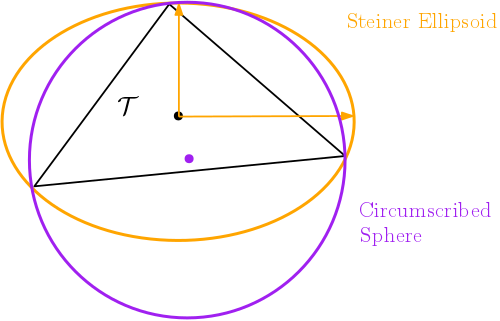
\includegraphics[scale=0.4]{ellipsoid_and_sphere}
	\caption{A simplex $\ssplx\subset\R^2$ and  its corresponding Steiner circumscribed ellipsoid in orange (light) and circumscribed sphere in purple (dark). The arrows illustrate the semi-axes of the ellipsoid.}
	\label{fig:ellipsoid_and_sphere}
\end{figure}

The appearance of the  eigenvalues  in  the semi-axes allows us to relate the volumes of $\El(\splx_G)$ and $\El(\splx_G^+)$.  The volume of an  ellipsoid in $\R^{n-1}$ written in the standard  form mentioned  above is 
\begin{equation*}
\frac{\pi^{\frac{n-1}{2}}}{\Gamma(\frac{n+1}{2})} \det(\bS^{-1}),
\end{equation*}
where $\Gamma(z)$ is the gamma function.  We emphasize  that the gamma function is distinct from $\Gamma_G$, the  total weight of spanning trees in $G$.  
For $\El(\splx_G)$, $\bS = \sqrt{\frac{n}{n-1}} \Eval^{-1/2}$, so 
\begin{align*}
\vol(\El(\splx_G)) &= \frac{\pi^{\frac{n-1}{2}}}{\Gamma(\frac{n+1}{2})} \bigg(\frac{n-1}{n}\bigg)^{\frac{n-1}{2}} \det\Eval^{1/2} \\
&= \frac{\pi^{\frac{n-1}{2}}}{\Gamma(\frac{n+1}{2})} \bigg(\frac{n-1}{n}\bigg)^{\frac{n-1}{2}}\bigg(\prod_{i<n}\lambda_i\bigg)^{1/2} \\
&= \frac{\pi^{\frac{n-1}{2}}}{\Gamma(\frac{n+1}{2})} \bigg(\frac{n-1}{n}\bigg)^{\frac{n-1}{2}} \sqrt{n}\Gamma_G^{1/2}.
\end{align*}

Moreover, as was noticed by Devriendt  and  Van Mieghem~\cite{devriendt2018simplex},  the linear dependence of both $\vol(\El(\splx_G)$ and $\vol(\splx_G)$ on $\Gamma_G^{1/2}$ (recall Corollary~\ref{cor:vol(SG)}) implies their ratio is independent of the particular graph $G$: 
\begin{equation*}
\frac{\vol(\El(\splx_G))}{\vol(\splx_G)} = \frac{\pi^{\frac{n-1}{2}}}{\Gamma(\frac{n+1}{2})} \bigg(\frac{n-1}{n}\bigg)^{\frac{n-1}{2}} \frac{(n-1)!}{\sqrt{n}}.
\end{equation*}

A similar procedure may be performed  with $\vol(\El(\splx_G^+))$  and $\vol(\splx_G^+)$. In that  case we  have 
\begin{align*}
\vol(\El(\splx_G^+)) = \frac{\pi^{\frac{n-1}{2}}}{\Gamma(\frac{n+1}{2})} \bigg(\frac{n-1}{n}\bigg)^{\frac{n-1}{2}} \det\Eval^{-1/2} = \frac{\pi^{\frac{n-1}{2}}}{\Gamma(\frac{n+1}{2})} \bigg(\frac{n-1}{n}\bigg)^{\frac{n-1}{2}} (n\Gamma_G)^{-1/2}.
\end{align*}
The ratio  of $\vol(\El(\splx_G^+))$ to $\vol(\splx^+_G)$ is the same as above. 



Next we investigate the circumscribed sphere of the combinatorial  simplex. Similarly to the circumscribed ellipsoid, the \emph{cirscumscribed sphere  of a convex body $\P$} is the sphere whose boundary contains all the vertices of $\P$. The circumscribed sphere does not exist in general. However, just as it is possible to always draw a circle containing the endpoints  of a triangle, so the circumscribed sphere of a hyperacute simplex always exists  as is demonstrated  by the following lemma.  

\begin{lemma}[\cite{fiedler1993geometric}]
	\label{lem:circ_sphere}
	Let $\splx^+\subset\R^{n-1}$ be a hyperacute simplex. The circumscribed sphere  of $\splx^+$ exists and is given by the set of points $\{\x:\x=\Sv\balpha, \; \la \balpha,\one \ra = 1, \; \la \balpha,\D\balpha\ra =0\}$, which is a sphere centred at the point $\frac{1}{2}\Sv(\L_G\bD + \one/n)$ with radius $\frac{1}{2}\sqrt{\bD^\tp\L_G\bD + 4\Rtot_G/n^2}$ where $G$ is $\splx^+$'s associated graph, and $\bD = \diag(\L_G^+(i,i))$. 
\end{lemma}

\begin{remark}
	It is no coincidence that the radius of the sphere is related to the top left entry in the  inverse of the Menger matrix  associated with  $\splx^+$. This was  noticed by Fiedler and is relied  upon in  the proof of Lemma~\ref{lem:circ_sphere}. 
\end{remark}


Until this point, we have been examining only the quadrics associated with the combinatorial simplices. We now consider the normalized simplices. Since all the vertices of the normalized simplex lie on the unit sphere, it's clear  that the circumscribed sphere of $\splxn_G$ is precisely $\{\x:\x^\tp\x=1\}$. It's not as straightforward  to see what they circumscribed ellipsoid, $\El(\splxn)$, is on the other hand. One might suspect that it obeys the  equation $\x^\tp \Svn^+(\Svn^+)^\tp=1-1/n$, as this is the natural analogue of \eqref{eq:steinerE}. However, because $\Svn^+$ and $\Svn$ obey a non-constant pseudoinverse relation, this equation fails the first test: $\svn_i^\tp\Svn^+(\Svn^+)^\tp\svn_i = \bchi_i^\tp(\I-\sqrt{\w}\sqrt{\w}^\tp/\vol(G))\bchi_i=1-\sqrt{w(i)w(j)}/\vol(G)$ is not constant. 
However, at this point we recall that beyond being simply  the inverse simplex of $\splx$, $\splx^+$ is also its dual.  We might thus hazard a guess that the correct matrix is $\Svn^\du (\Svn^\du)^\tp$, where $\Svn^\du$ is the vertex matrix of $\splxn^\du$. The  following lemma  confirms this hypothesis and, moreover, verifies that similar reasoning can be applied to the Steiner Ellipsoid of any simplex---not only those corresponding to graphs.  

\begin{lemma}
	\label{lem:El(T)_general}
	Let $\ssplx\subset\R^{n-1}$ be a simplex whose dual has vertex matrix  $\Sv^\du$. Then  the Steiner ellipsoid of $\ssplx$ is 
	\begin{equation*}
	\El(\ssplx) = \bigg\{\x:\x^\tp\Sv^\du(\Sv^\du)^\tp\x=\frac{n-1}{n}\bigg\}.
	\end{equation*} 
\end{lemma}

\begin{proof}
	The computation is almost identical to that in the proof of Lemma~\ref{lem:El(S)}, except we  take $\M=\Sv^\du(\Sv^\du)^\tp$ and use the general relationship between  $\Sv^\tp\Sv$ and $\Sv^\du(\Sv^\du)^\tp$ given by Lemma~\ref{lem:dual_pseudoinverse}. 
\end{proof}


\section{Resistive Polytope}
\label{sec:resistive_polytope}
In this section we explore the relationship between the inverse combinatorial simplex of $G$ and another geometric object related to the effective resistance of the graph. Consider the vertices $\bmu_i=\L_G^{+/2}\bchi_i\in\R^n$, for $i\in[n]$. This yields $n$ points in $\R^n$, also with pairwise squared distances equal to the effective resistance of the graph: 

\begin{equation*}
\norm{\bmu_i-\bmu_j}_2^2 = \norm{\L_G^{+/2}(\bchi_i-\bchi_j)}_2^2 =  (\bchi_i-\bchi_j)^\tp \L_G^+(\bchi_i-\bchi_j)=\effr(i,j).
\end{equation*}

This embedding has been referred to as a \emph{resistive embedding}~\cite{shayanNotes,ding2011cover}, and is an example of an $\ell_2^2$ metric~\cite{arora2009expander} owing  to the well known fact that the effective resistance is a metric (e.g., ~\cite{klein1993resistance}). That being said however, while the mapping seems to be known~\cite{ghosh2008minimizing}, there is very little literature on its properties. 

Set 
\begin{equation}
\label{eq:res_pol}
\respol_G \equiv \conv(\{\bmu_i\}),
\end{equation}
and  call  $\respol_G$ the \emph{resistive polytope of $G$}. Note that $\L_G^{+/2}$ is $\respol_G$'s vertex matrix. As usual, we may omit the subscript $G$ for convenience. We emphasize that while the vertices $\{\bmu_i\}$ obey the same pairwise  distances as  those of the inverse simplex $\splx_G^+$, $\respol_G$  is not the same object as $\splx_G^+$. First, of course, there is  the fact that it sits in  $\R^n$. However,  we also note that the entries of $\mu_i$ (the first $n-1$, at least) do not match those of $\sv_i^+$. Indeed, 

\begin{align*}
\mu_i(\ell) = \L_G^{+/2}(\ell,i) = \sum_{j\in[n]}\lambda_j^{-1/2}\vp_j\vp_j^\tp(\ell,i) = \sum_{j\in[n]}\lambda_j^{-1/2}\vp_j(\ell)\vp_j(i).
\end{align*}
Recalling the formula for the vertices of the inverse simplex $\splx^+$ demonstrates that 
\begin{equation*}
\mu_i(\ell) = \sum_{j\in[n]}\sv_\ell^+(j)\vp_j(i) = \sum_{j\in[n]}\sv_i^+(j)\vp_j(\ell).
\end{equation*}
Hence, in general, $\mu_i(\ell)\neq \sv_i^+(\ell)$. However, the dot product between the vertices of $\respol_G$ does respect  the same relationships as those between the vertices of $\splx_G^+$:
\begin{align*}
\la \bmu_i,\bmu_j\ra &=\sum_{\ell\in[n]} \L_G^{+/2}(\ell,i)\L_G^{+/2}(\ell,j) \\
&= \la \L_G^{+/2}(\cdot,i),\L_G^{+/2}(\cdot,j)\ra \\
&=\la \L_G^{+/2}(\cdot,i),\L_G^{+/2}(j,\cdot)\ra= \L_G^+(i,j),
\end{align*}
since $\L_G^{+/2}$ is symmetric and  $\L_G^{+/2}\L_G^{+/2}=\L_G^+$.  We can also see this from recalling that 
\[\effr(i,j) = \L_G^+(i,i) + \L_G^+(j,j) - \frac{1}{2}\L_G^+(i,j),\]
combined with the facts that $\norm{\bmu_i-\bmu_j}_2^2 = \effr(i,j)$ and $\norm{\bmu_i}_2^2 = \L_G^+(i,i)$. The centroid of $\re_G$ also coincides with the origin  of $\R^n$: 
\begin{equation*}
\cent(\re_G) = \frac{1}{n}\L_G^{+/2}\one = \frac{1}{n}\sum_{i\in[n-1]}\lambda_i^{-1/2}\vp_i\vp_i^\tp \one = \zero.
\end{equation*}

One therefore begins to suspect that $\respol_G$ is the same object of  $\splx_G^+$, simply projected onto some hyperplane of $\R^n$. The following lemma  demonstrates that this is indeed the  case, and  that  the hyperplane  is that which is has $\spn(\one)$ as its orthogonal complement. See Figure~\ref{fig:res_embedding} for an  illustration. 

\begin{lemma}
	The all ones vector is orthogonal to $\re_G$. 
\end{lemma}
\begin{proof}
	We need to show that for all $\p,\q\in\re_G$, $\la \one,\p-\q\ra=0$. As usual, let $\x$ and $\y$ be the barycentric coordinates of $\p$ and $\q$ so that $\p=\L_G^{+/2}\x$ and $\q=\L_G^{+/2}\y$. We have
	\begin{align*}
	\la \one,\p\ra &= \sum_{\ell\in[n]} (\L_G^{+/2}\x)(\ell) = \sum_{\ell\in[n]} \sum_{j\in [n]}\L_G^{+/2}(\ell,j)x(j) = \sum_{j\in[n]}x(j) \sum_{\ell\in[n]}\L_G^{+/2}(\ell,j),
	\end{align*}
	where for any $j$, 
	\[\sum_{\ell\in[n]}\L_G^{+/2}(\ell,j)= \one^\tp \L_G^{+/2}\bchi_j=\sum_{\ell\in[n-1]} \lambda_\ell^{-1/2}\one^\tp \vp_\ell\vp_\ell^\tp\bchi_j=0,\]
	since $\vp_i\in\spn(\one)^\perp$  for all $i<n$. Hence  $\la \one,\p\ra=0$ meaning that $\la \one,\p-\q\ra=0$ as well. 
\end{proof}

\begin{figure}
	\centering
	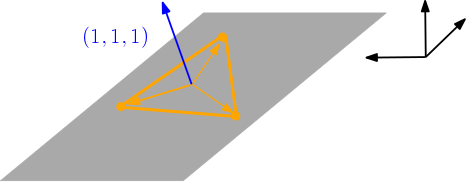
\includegraphics[scale=0.5]{res_embedding}
	\caption{The resistive embedding (in orange;  light) of a graph with three nodes sits in a plane (gray) which is parallel to the all ones vector. }
	\label{fig:res_embedding}
\end{figure}

The relationship between $\re$ and $\splx$ gives us an alternate way to prove equalities such as \eqref{eq:c(S_U)}: There exists an isometry\footnote{A distance preserving map.} between $\re$ and $\splx$, so 
\begin{equation*}
\norm{\cent(\splx^+_U)}_2^2 = \norm{\cent(\re_U)}_2^2 = \frac{1}{|U|^2} \norm{\L_G^{+/2}\bchi_U}_2^2 = \frac{1}{|U|^2}w(\delta^+ U).
\end{equation*}


Additionally, just as $\splx_G^+$  has  the inverse $\splx_G$, $\respol_G$  has an inverse which respects the same  relationships. As one might guess, this inverse has vertex matrix $\L_G^{1/2}$. To see this, for any $i,j\neq k$,  we have 
\begin{equation*}
\la \L_G^{1/2}\bchi_i,\L_G^{+/2}\bchi_j-\L_G^{+/2}\bchi_k\ra = \bchi^\tp \L_G^{1/2}\L_G^{+/2}(\bchi_j-\bchi_k)\ra,
\end{equation*}
where 
\begin{align*}
\L_G^{1/2}\L_G^{+/2} &= \sum_{r,s=1}^{n-1}\lambda_r^{1/2}\lambda_s^{-1/2}\vp_r\vp_r^\tp\vp_s\vp_s^\tp = \sum_{r=1}^{n-1} \vp_r\vp_r^\tp,
\end{align*}
and 
\begin{align*}
\sum_{r=1}^{n-1}\bchi_i \vp_r\vp_r^\tp\bchi_j = \sum_{r=1}^{n-1}\vp_r(i)\vp_r(j) = \delta_{ij} - \frac{1}{n},
\end{align*}
using Equation \eqref{eq:sum_double_ortho}. Hence, 
\begin{align*}
\bchi_i^\tp \L_G^{1/2}\L_G^{+/2}(\bchi_j-\bchi_k) = \delta_{ij} - \frac{1}{n} - (\delta_{ik}-\frac{1}{n}) = \delta_{ij}.
\end{align*}

To  conclude, there exists an isometry between the inverse combinatorial  simplex of a graph $G$ (which  lies in $\R^{n-1}$) and the effective  polytope, $\re_G$ of  $G$ (which  lies in $\R^n$). The resistive polytope lies in a hyperplane orthogonal to the  all-ones vector.  



%\section{Effective  Resistance  \&  Dynamics}
%\label{sec:dynamics}
%In this section we briefly highlight a few connections between stochastic process on $G$ and  the geometry of its inverse combinatorial simplex $\splx_G^+$. 



\section{Continuous Time Random Walks}
\label{sec:random_walks}
This current section is for the reader who is less interested  in the  mathematics  behind the graph-simplex correspondence, and is reading only for the vague  hope  that some of the underlying geometry will be aesthetically pleasing. While  the  content has certainly failed in this vein thus far, this section  is the closest we will come to remedying the situation. 

Consider a  random walk on a graph. The probability distribution  governing the dynamics is a barycentric  coordinate: each coordinate is non-negative and they sum to one. Therefore, we can represent the probability distribution as a point in the simplex and the probability  distribution as a function of time as a path in the simplex. See Figure~\ref{fig:random_walk} for an illustration. In what follows we give equations which determine the dynamics of the path in the simplex as a function of the eigenvalues  and eigenvectors  of the graph. 

We will examine a continuous time random walk which  obeys the equation 
\begin{equation*}
\frac{d \bpi(t)}{dt } = -\L_G\W_G^{-1/2} \bpi(t),
\end{equation*}
and has the solution $\bpi(t)  = \exp(-\L_G\W_G^{-1/2}t)\bpi(0)$. This, however, is relatively unsightful in terms of  analyzing the dynamics of $\bpi(t)$ in terms of the  graph.  Instead, in  what follows we seek  to develop a solution to $\bpi(t)$ in terms of the  eigendecomposition of  $G$.  Define $\bpi_1(t) = \W^{-1/2}\bpi(t)$ and $\bpi_2(t) = \Eign^\tp \bpi_1(t)$, where we recall that $\Eign^\tp$ is the eigenvector matrix  of  $\Ln_G$.  Then 
\begin{equation*}
\frac{d \bpi_1(t)}{dt} = \W^{-1/2}\frac{d \bpi(t)}{dt} = -\W^{-1/2}\L_G\W^{-1/2}\W^{-1/2}\bpi(t) = - \Ln_G\bpi_1(t),
\end{equation*}
and, using the eigendecomposition of $\Ln_G$,   
\begin{equation*}
\frac{ d\bpi_2(t)}{dt} = \Eign^\tp \frac{d\bpi_1(t)}{dt} = -\Eign^\tp \Ln_G \bpi_1(t) = -\Eign^\tp \Eign\Evaln\Eign^\tp \bpi_1(t) = -\Evaln  \bpi_2(t),
\end{equation*}
since  $\Eign^\tp\Eign=\I$. This equation  has the solution 
\begin{equation*}
\bpi_2(t) = \exp(-\Evaln t)\bpi_2(0) = \begin{pmatrix}
e^{-\lambda_1 t}  & &\\
& \ddots  & \\
&& e^{-\lambda_{n-1} t}
\end{pmatrix}  \bpi_2(0).
\end{equation*}

\begin{figure}
	\centering
	\begin{minipage}{0.32\textwidth}
		\centering
		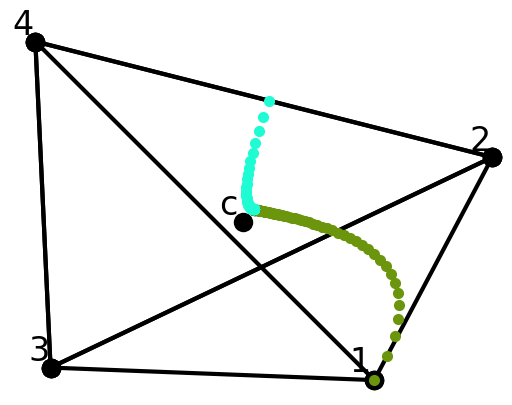
\includegraphics[scale=0.6]{dynamics1}
		\subcaption{}
	\end{minipage}
	\begin{minipage}{0.32\textwidth}
		\centering
		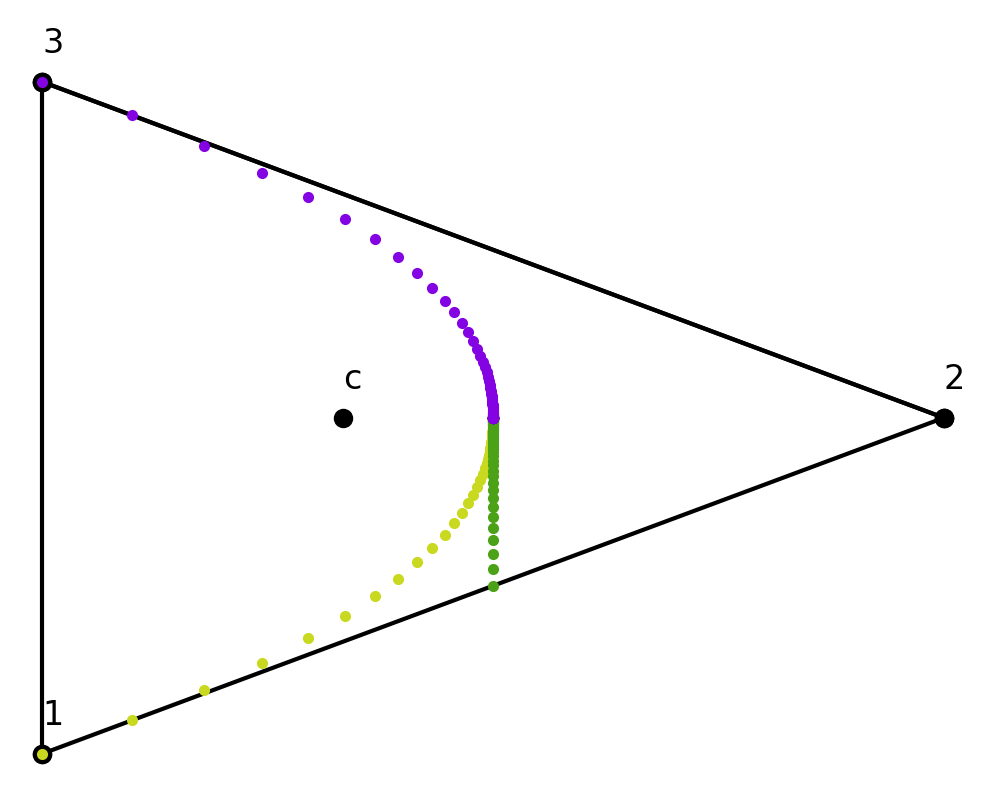
\includegraphics[scale=0.4]{dynamics3}
		\subcaption{}
	\end{minipage}
	\begin{minipage}{0.32\textwidth}
		\centering
		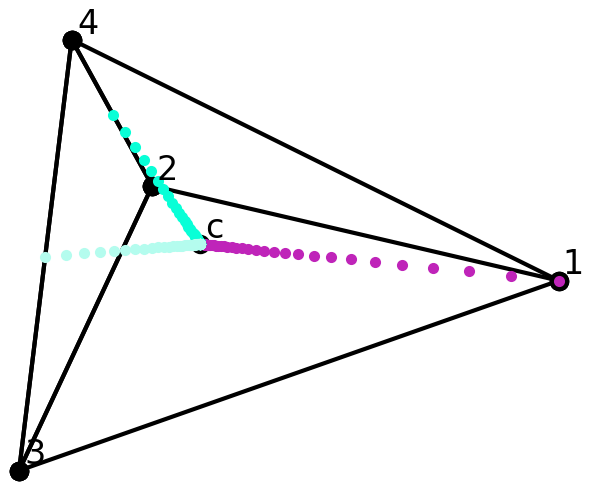
\includegraphics[scale=0.6]{dynamics2}
		\subcaption{}
	\end{minipage}
	\caption{Random walk dynamics plotted as points  in the simplex. Figures (a) and (b) are plotted using the normalized simplex;  figure (c) uses  the normalized simplex. The  underlying graph of Figure (a) has edges $(1,2)$, $(2,3)$, $(3,4)$, $(2,4)$, that underlying (b) edges $(1,2)$ and $(2,3)$ and that of (c) is the complete graph  $K_4$. }
	\label{fig:random_walk}
\end{figure}

Combining the  definitions of $\bpi_1$  and $\bpi_2$ gives $\bpi_2(t)  = \Eign^\tp \bpi_1(t) = \Eign^\tp \W^{-1/2}\bpi(t)$, hence 
$\bpi(t) = \W^{1/2} \Eign \bpi_2(t)$. As a point in the  simplex this gives 
\begin{equation*}
\p(t)  = \Sv\bpi(t) = \Eval^{1/2}\Eig^\tp \W^{1/2}\Eign \bpi_2(t) = \Y\bpi_2(t),
\end{equation*}
after defining $\Y\equiv \Eval^{1/2}\Eig^\tp \W^{1/2}\Eign$. As a point in the normalized simplex, we have 
\begin{equation*}
\q(t) = \Svn\bpi(t) = \Evaln^{1/2}\Eign^\tp\W^{1/2}\Eign\bpi_2(t) = \Yn\bpi_2(t),
\end{equation*}
where $\Yn= \Evaln^{1/2}\Eign^\tp\W^{1/2}\Eign$. We thus  see that the matrices 
\begin{equation*}
\Y = \begin{pmatrix}
\lambda_1^{1/2}\sum_{i\in[n]} \vp_1(i)\vpn_1(i) w_i^{1/2} & \dots &  \lambda_1^{1/2}\sum_{i\in[n]} \vp_1(i)\vpn_{n-1}(i) w_i^{1/2} \\
\vdots & \ddots & \vdots \\
\lambda_{n-1}^{1/2}\sum_{i\in[n]} \vp_{n-1}(i)\vpn_1(i) w_i^{1/2} & \dots &  \lambda_{n-1}^{1/2}\sum_{i\in[n]} \vp_{n-1}(i)\vpn_{n-1}(i) w_i^{1/2} 
\end{pmatrix},
\end{equation*}
and  
\begin{equation*}
\Yn  = \begin{pmatrix}
\lambdan_1^{1/2}\sum_{i\in[n]} \vpn_1(i)\vpn_1(i) w_i^{1/2} & \dots &  \lambdan_1^{1/2}\sum_{i\in[n]} \vpn_1(i)\vpn_{n-1}(i) w_i^{1/2} \\
\vdots & \ddots & \vdots \\
\lambdan_{n-1}^{1/2}\sum_{i\in[n]} \vpn_{n-1}(i)\vpn_1(i) w_i^{1/2} & \dots &  \lambdan_{n-1}^{1/2}\sum_{i\in[n]} \vpn_{n-1}(i)\vpn_{n-1}(i) w_i^{1/2} 
\end{pmatrix},
\end{equation*}
govern the dynamics of the random walk in  $\splx_G$ and $\splxn_G$, respectively.  More specifically, letting $\Y=(\y_1\;\dots\;\y_n)$ we have 
\[\p(t) = \sum_{i\in[n-1]} \y_i (\bpi_2(t))(i) = \sum_{i\in[n-1]}  \y_i e^{-\lambda_i t} \Eign^\tp \W^{-1/2}\bpi(0)(i),\]
and a similar  equation for $\q(t)$. 






